\section{Problem Statement}
The produced water re-injection facility considered in this study is represented as a network in Figure~\ref{}. The network is represented by a set of nodes $\mathcal{J}$ that are interconnected by a set of arcs $\mathcal{L}$. The set of nodes $\mathcal{L}$ are subdivided into a set of tanks $\mathcal{J}_T$; a set of junctions $\mathcal{J}_J$; a set of injection wells $\mathcal{J}_W$; and a set of ocean discharge $\mathcal{J}_D$. The set of arcs $\mathcal{L}$ are also subdivided into a set of valves $\mathcal{L}_V$; a set of pipelines $\mathcal{L}_P$; a set of fixed-speed pumps $\mathcal{L}_{FSP}$; and  a set of variable-speed pumps $\mathcal{L}_{VSP}$. Its graphical representation can be found in Figure \ref{fig:facility}.
\begin{figure}
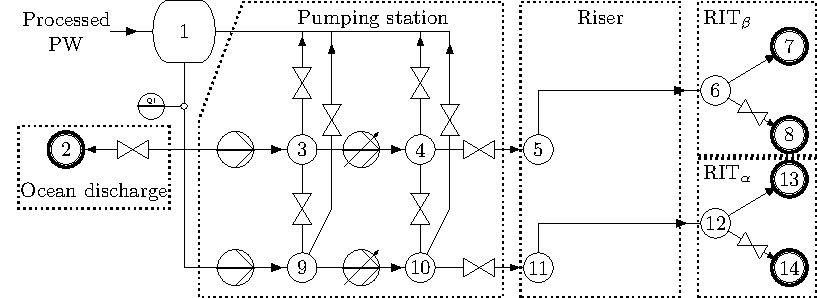
\includegraphics[]{PWRI_full_facility.pdf}
\end{figure}

\par One can see that this network present the following characteristics: (i) Looped layout; (ii) a pumping train is present upstream of each sink injection well; (iii) each train have fixed and variable speed pumps in series, and (iv) control valves are located upstream of each sink injection well. 
\par The considered network can be described by the set of differential algebraic equations (DAE) shown below, 
\begin{subequations}\label{dae:continuous}
    \begin{alignat}{2}
        \dot{x}(t)& =  f(x(t),{z}(t),{u}(t),b(t),w(t)),\label{dae:dynamic}
        \\
        0& = g(x(t),z(t),u(t),b(t),w(t)), \label{dae:algebraic}
    \end{alignat}
with nonlinear maps given by $f:\mathbb{R}^{n_x}\times\mathbb{R}^{n_z}\times\mathbb{R}^{n_u}\times\{0,1\}^{n_b}\times\mathbb{R}^{n_w}\rightarrow{\mathbb{R}^{n_x}}$, and $g:\mathbb{R}^{n_x}\times\mathbb{R}^{n_z}\times\mathbb{R}^{n_u}\times\{0,1\}^{n_b}\times\mathbb{R}^{n_w}\rightarrow{0}$. Moreover, ${x}\in\mathbb{R}^{n_x}$ are dynamic states, ${z}\in{\mathbb{R}}^{n_z}$ are algebraic states, ${u\in\mathbb{U}\in{\mathbb{R}}^{n_u}}$ are control inputs, $b\in\{0,1\}^{n_b}$ are binary control inputs, and $w\in{\mathbb{R}^{n_w}}$ are disturbances. 
\end{subequations}
% The system is augmented with measurement output as follows,
% \begin{align}\label{dae:measurement}
%     c(t) &= h_c(x(t), z(t), w(t)), 
%     \\
%     q(t) &= h_q(x(t), z(t), u(t), b(t), w(t)), 
% \end{align}
% \end{subequations}
% where the output maps are given as $h_c:\mathbb{R}^{n_x}\times\mathbb{R}^{n_z}\times\mathbb{R}^{n_w}\rightarrow\mathbb{R}_{\geq 0}$, and $h_q:\mathbb{R}^{n_x}\times\mathbb{R}^{n_z}\times\mathbb{R}^{n_u}\times\{0,1\}^{n_b}\times\mathbb{R}^{n_w}\rightarrow \mathbb{R}_{\geq 0}$, with $c\in\mathbb{R}_{\geq 0}$, and $q\in\mathbb{R}_{\geq 0}$ as concentration and flowrate outputs, respectively. Measurements of the system are assumed to be performed regularly. 
% \par We define the expanding-time FWMC as a time-based weighted average evaluated from a fixed initial time $t_m$, to a variable final time $t$. The expanding-time FWMC is shown below,
% \begin{subequations}
%     \begin{equation}
%         \tilde{c}(t_m,t)
%         = \frac{\mathbf{M}(t_m,t)}{\mathbf{V}(t_m,t)}, \label{eq:expanding_FWMC}
%     \end{equation}
%     with,
%         \begin{alignat}{2}
%             \mathbf{M}(t_m,t)&=\int_{t_m}^{t} {c}(\tau){q}(\tau) d\tau,
%             \\ 
%             \mathbf{V}(t_m,t)&=\int_{t_m}^{t} {q}(\tau)~d\tau, \label{fwmc:volume}
%         \end{alignat}
% \end{subequations}
% where $\mathbf{M}:\mathbb{R}_{\geq{0}}\rightarrow{\mathbb{R}_{\geq{0}}}$ and $\mathbf{V}:\mathbb{R}_{\geq{0}}\rightarrow{\mathbb{R}_{\geq{0}}}$ are named as the total load map and the total volume map, respectively. Based on the expanding-time FWMC, we define the fixed-time FWMC, $\tilde{c}(t_m,t_{m+1})\in\mathbb{R}$, which has a fixed initial and final time of integration.
% \par We use the previous definitions given for the expanding-time FWMC, and the fixed-time FWMC to create what we refer to as the piecewise expanding-time FWMC\@:
% \begin{equation}\label{eq:semi_continuous_FWMC}
%     \tilde{c}(t)
%     = \left\{\begin{array}{lr}
%         \tilde{c}(t_m,t), & \text{for } t_m<{t}\leq{t_{m+1}}
%     \end{array}\right\}, \quad
%     \forall{m} \in{\mathbb{N}},
% \end{equation}
% where ${\tilde{c}(t)\in\mathbb{R}}$ is the piecewise expanding-time FWMC\@. Each fixed-time FWMC segment has a time interval ${\Delta T_m=t_{m+1}-t_{m}}$, which is a few orders of magnitude longer than the settling time of system~\eqref{dae:continuous}. The first goal is to have the fixed-time FWMCs constrained in a particular region:
% \begin{equation}\label{dae:FWMC_bound}
%     \tilde{c}(t_m,t_{m+1}) \in \mathbb{C}_f, \quad \forall{m}\in{\mathbb{N}}.
% \end{equation} 
% \par The system represented by~\eqref{dae:continuous},~\eqref{eq:semi_continuous_FWMC}, and~\eqref{dae:FWMC_bound} is accompanied by a discontinuous stage cost of the form $\ell:\mathbb{R}^{n_x}\times\mathbb{R}^{n_z}\times\mathbb{R}^{n_u}\times\{0,1\}^{n_b}\to\mathbb{R}$. Discontinuity comes from the binary variables $b(t)$, which contains elements representing on/off status of pumping systems. Changes between these statuses are generally accounted as additional costs in $\ell(x(t),z(t),u(t),b(t))$~\cite{}. Thus, the second goal is to  minimize the stage cost $\ell(x(t),z(t),u(t),b(t))$.
The system represented by~\eqref{dae:continuous} is accompanied by a discontinuous stage cost of the form $\ell:\mathbb{R}^{n_x}\times\mathbb{R}^{n_z}\times\mathbb{R}^{n_u}\times\{0,1\}^{n_b}\to\mathbb{R}$.

The facility model as well as its performance metrics are represented in the following subsections.
% Discontinuity comes from the binary variables $b(t)$, which contains elements representing on/off status of pumping systems.
\par Before introducing the facility model, we list the assumptions considered in this work. 
\begin{itemize}
    \item Produced water (PW) is considered an incompressible fluid and its temperature is assumed be constant. Moreover, oil content in PW density is neglected. Furthermore, we assume an isothermal process. As a consequence, the PW specific weight $\gamma_i$ is considered constant.
    \item ...
    \item ...
\end{itemize}
% \subsection{Simulation - Variables}
% In this subsection, we define the variables that are part of the DAE system shown in~\eqref{dae:continuous}.  




\subsection{Nodes - Mathematical representation}
    \par Each node is associated with a set of variables and equations that enables one to represent their behavior. Below, we present the variables that describe the set of tanks $\mathcal{L}_T$:
    \begin{subequations}
        \begin{alignat}{2}
            x_i &= \left[\begin{array}{c}
                V_i
            \end{array}\right], &\forall i \in \mathcal{J}_T\\
            z_i &= \left[\begin{array}{cc}
                H_i & h_i
            \end{array}\right], &\forall i \in \mathcal{J}_T\\
            p_i &= \left[\begin{array}{cccc}
                d_i & z_i & P_i^s
            \end{array}\right], &\forall i \in \mathcal{J}_T
        \end{alignat}    
    \end{subequations}
    where $V_i$ is liquid volume at node $i$; $H_i$ is the hydraulic head at node $i$; $h_i$ is the PW level at node $i$; $d_i$ is the demand flowrate at node $i$; $z_i$ is the elevation at node $i$; and $P_i^s$ is the surface pressure at node $i$. The set of junctions $\mathcal{J}_J$ are associated with the following variables,
    \begin{subequations}
    \begin{alignat}{2}
        z_i &= \left[\begin{array}{c}
            H_i
        \end{array}\right], &\forall i \in \mathcal{J}_J \\
        p_i &= \left[\begin{array}{ccc}
            z_i
        \end{array}\right], &\forall i \in \mathcal{J}_J.
    \end{alignat}
    \end{subequations}
    The variables that describe the set of injection wells $\mathcal{J}_W$ are shown below,
    \begin{subequations}
    \begin{alignat}{2}
        z_i &= \left[\begin{array}{ccc}
            H_i & P_i & d_i
        \end{array}\right], & \forall i \in \mathcal{J}_W \\
        p_i &= \left[\begin{array}{ccc}
            P_i^r & J_i & z_i
        \end{array}\right], & \forall i \in \mathcal{J}_W
    \end{alignat}
    \end{subequations}
    where $P_i^r$ \textit{is the reservoir pressure} at node $i$; and $J_i$ is the injectivity index at node $i$. Finally, for the set of ocean discharge $\mathcal{J_D}$, we have considered the following variables:
    \begin{subequations}
    \begin{alignat}{2}
        z_i &= \left[\begin{array}{ccc}
            H_i & d_i
        \end{array}\right], & \forall i \in \mathcal{J}_D \\
        p_i &= \left[\begin{array}{cc}
            P_i & z_i
        \end{array}\right], & \forall i \in \mathcal{J}_D.
    \end{alignat}
    \end{subequations}
    \par Mass balance equations are responsible for guaranteeing that continuity holds in each node $\mathcal{L}$. We stress that only tank nodes $\mathcal{J}_T$ presents dynamics for the volume of liquid, as seen below,
    \begin{subequations}
        \begin{alignat}{2}
            \dot{V}_{i} &= \sum_{\underset{j\in\mathcal{J}}{i \neq j}}\left(q_{(i,j)} - q_{(j,i)}\right) - d_{i},& \forall i \in \mathcal{J}_T \label{tank:mass_balance}
            \\
            0 &= \sum_{\underset{j\in\mathcal{J}}{i \neq j}}\left(q_{(i,j)} - q_{(j,i)}\right), & \quad \forall i \in \mathcal{J}_J \label{junction:mass_balance}
            \\
            0 &= \sum_{\underset{j\in\mathcal{J}}{i \neq j}}\left(q_{(i,j)} - q_{(j,i)}\right) - d_{i}, &\quad \forall i \in \mathcal{J}_D \cup \mathcal{J}_W\label{source_sink:mass_balance}
        \end{alignat}
    \end{subequations}
    where $q_{(i,j)}$ is the flowrate at arc ${(i,j)}$. Furthermore, \eqref{tank:mass_balance} is the mass balance at tank nodes $\mathcal{J}_T$; 
    \eqref{junction:mass_balance} is the mass balance at junction nodes $\mathcal{J}_J$;
    and \eqref{source_sink:mass_balance} is the mass balance at ocean discharge and well nodes $\mathcal{J}_D \cup \mathcal{J}_W$. Furthermore, we employ the convention that positive values of demand represents PW leaving the node, while positive is for PW entering the node. 
    \par It is considered that each node $\mathcal{J}$ holds an amount of mechanical energy. This energy is represented in terms of hydraulic head,
    \begin{subequations}
        \begin{alignat}{2}
            H_i &= \frac{P_i^s}{\gamma_i} + \left(z_i + h_i - z_0 \right), &\quad \forall i \in \mathcal{J}_T \label{tank:hydraulic_head}
            \\ 
            H_i &= \frac{P_i}{\gamma_i} + \left(h_i - z_0 \right), &\quad \forall i \in \mathcal{J}\setminus\mathcal{J}_T, \label{non-tank:hydraulic_head}
        \end{alignat}    
    \end{subequations}
    in which~\eqref{tank:hydraulic_head} is the hydraulic head at tank nodes $\mathcal{J}_T$; and~\eqref{non-tank:hydraulic_head} is the hydraulic head at non-tank nodes $\mathcal{J}\setminus\mathcal{J}_T$. 
    \par A relation known as inflow performance relationship (IPR) correlates the pressure and flowrate at well nodes $\mathcal{J}_W$. The IPR can be obtained experimentally by performing injectivity tests in each particular well. For water, the IPR can be assumed to be linear.
    \begin{alignat}{2}
        P_i & = P^r_i + \frac{d_i}{J_i}, & \quad \forall i \in \mathcal{J}_W, \label{well:IPR}
    \end{alignat}
    in which~\eqref{well:IPR} is the IPR in well nodes $\mathcal{J}_W$.
    % h_i &= f(V_i), \label{tank:level}
    % \par The degasser is represented by the set of equations shown below,
    % \begin{alignat}{2}
    %     \dot{V}_{i} &= \sum_{\underset{j\in\mathcal{J}}{i \neq j}}\left(q_{(i,j)} - q_{(j,i)}\right) + q_{(i,i)},\label{tank:mass_balance}
    %     \\
    %     H_i &= \frac{p_i^s}{\gamma_i} + \left(z_i + h_i - z_0 \right), \label{tank:hydraulic_head}
    %     \\ 
    %     h_i &= f(V_i), \label{tank:level}
    % \end{alignat}
    % in which~\eqref{tank:mass_balance} is the mass balance of PW in the tank;~\eqref{tank:hydraulic_head} is the hydraulic head at the surface of the PW in the tank; and~\eqref{tank:level} is the relation between liquid volume and level. 
\subsection{Arcs - Mathematical representation}
    \par Each arc is represented by a set of variables and equations to describe their behavior. The variables that represent the set of vales $\mathcal{L}_V$ are given as,
    \begin{subequations}
        \begin{alignat}{3}
            z_{(i,j)} &= \left[\begin{array}{ccc}
                q_{(i,j)} & H^L_{(i,j)}
            \end{array}\right],  & \forall i \in \mathcal{L}_V, \\
            u_{(i,j)} &= \left[\begin{array}{ccc}
                \phi_{(i,j)}
            \end{array}\right],  & \forall i \in \mathcal{L}_V, \\
            p_{(i,j)} &= \left[\begin{array}{cc}
                K_{(i,j)}
            \end{array}\right], & \forall i \in \mathcal{L}_V,
        \end{alignat}
    \end{subequations}
    in which $\phi_{(i,j)}$ is the valve opening; and $H^L_{(i,j)}$ is the hydraulic head loss at arc ${(i,j)}$. The variables that describe the set of pipelines are shown below,
    \begin{subequations}
        \begin{alignat}{2}
            z_{(i,j)} &= \left[\begin{array}{ccc}
                q_{(i,j)} & H^L_{(i,j)}
            \end{array}\right], & \forall i \in \mathcal{L}_P,
            \\
            p_{(i,j)} &= \left[\begin{array}{ccc}
                C_{(i,j)} & \Delta s_{(i,j)} & D_{(i,j)}
            \end{array}\right], & \forall i \in \mathcal{L}_P,
        \end{alignat}
    \end{subequations}
    $C_{(i,j)}$ is the Hazen-William constant at arc ${(i,j)}$;
    $\Delta s_{(i,j)}$ is the pipeline length at arc ${(i,j)}$;
    and $D_{(i,j)}$ is the pipeline diameter at arc ${(i,j)}$. 
    To represent the set of FSPs $\mathcal{L}_{FSP}$, we consider the following variables,
    \begin{subequations}
        \begin{alignat}{2}
            z_{(i,j)} &= \left[\begin{array}{cccc}
                q_{(i,j)} & H^G_{(i,j)} & W_{(i,j)} & \eta_{(i,j)}
            \end{array}\right], & \forall i \in \mathcal{L}_{FSP},
            \\
            b_{(i,j)} &= \left[\begin{array}{c}
                Z_{(i,j)}
            \end{array}\right], & \forall i \in \mathcal{L}_{FSP},
            \end{alignat}
    \end{subequations}
    where $H^G_{(i,j)}$ is the hydraulic head gain at arc ${(i,j)}$; 
    and $Z_{(i,j)}$ is the pump on/off status at arc ${(i,j)}$. 
    Finally, the variables that describe the set of VSPs $\mathcal{L}_{VSP}$ can be found below:
    \begin{subequations}
        \begin{alignat}{2}
            z_{(i,j)} &= \left[\begin{array}{cccc}
                q_{(i,j)} & H^G_{(i,j)} & W_{(i,j)} & \eta_{(i,j)}
            \end{array}\right], & \forall i \in \mathcal{L}_{VSP}  
            \\
            u_{(i,j)} & = \left[\begin{array}{c}
                \omega_{(i,j)}
            \end{array}\right], & \forall i \in \mathcal{L}_{VSP}  
            \\
            b_{(i,j)} &= \left[\begin{array}{ccc}
                Z_{(i,j)}
            \end{array}\right], & \forall i \in \mathcal{L}_{VSP}
            \end{alignat}
    \end{subequations}
    where $\omega_{(i,j)}$ is the pump rotation at arc $(i,j)$.
    \par At each arc it is necessary to account for gains or losses of mechanical energy. The mechanical energy balance is performed in terms of hydraulic head and is shown below,
    \begin{subequations}
        \begin{alignat}{3}
            H^L_{(i,j)} &= H_{j} - H_{i}, && \forall (i,j) \in \mathcal{L}_{V} \cup \mathcal{L}_{P}, \label{pipeline_valve:hydraulic_head_balance}
            \\
            Z_{(i,j)}H^G_{(i,j)} &= Z_{(i,j)}\left(H_{i} - H_{j}\right), && \forall (i,j) \in \mathcal{L}_{FSP}\cup \mathcal{L}_{VSP},\label{pumps:hydraulic_head_balance}
        \end{alignat}
    \end{subequations}
    in which \eqref{pipeline_valve:hydraulic_head_balance} is the mechanical energy balance for valves and pipelines; and \eqref{pumps:hydraulic_head_balance} is the mechanical energy balance at FSP and VSP nodes, which must hold when pump $(i,j)$ is on.
    \par As PW passes through pipeline arcs $\mathcal{L}_P$, friction is exerted on the fluid by the inner pipeline wall, and part of the energy content of the fluid dissipates. For a single-phase system, the relation between hydraulic head loss and friction can be given by the Darcy-Weisbach empirical relation. However, .... Due to that, we consider in this work the Hazen-William empirical equation.
    Moreover, it is known that PW flows from a node with higher hydraulic head to one with lower hydraulic head. Due to that, we do not restrict the flowrate to only positive values in pipelines \citep{Gleixner2012}. One way of representing this behavior is by introducing non-smooth constraints, and is shown below:
    \begin{alignat}{2}
        H^L_{(i,j)} &= 
            \frac{10.67 \gamma_{(i,j)} \Delta s_{(i,j)}}{{C_{(i,j)}}^{1.852}{d_{(i,j)}}^{4.87}} sgn(q_{(i,j)})|q_{(i,j)}|^{1.852}, \label{pipeline:hazen_william}
    \end{alignat}
    in which \eqref{pipeline:hazen_william} is the Hazen-Willian equation for hydraulic loss. 
    \par Control valves enables one to regulate the flowrate of the PW. Assuming turbulent flow throug control valves, its mathematical formulation is given below~\citep{Fisher2005},
    \begin{equation}
        q_{(i,j)} =  27.3 \phi_{(i,j)} K sgn(H^L_{(i,j)})\sqrt{\frac{|H^L_{(i,j)}|g}{10^5}}, \quad \forall {(i,j)} \in \mathcal{L}_V \label{valve:hydraulic_loss}
    \end{equation}
    in which $sgn(H^L_{(i,j)})$ accounts for the possibility of reverse flow through valves. It is important to notice in~\eqref{valve:hydraulic_loss} that when a valve is closed, decoupling between $H^L_{(i,j)}$ and $q_{(i,j)}$ occurs and $H^L_{(i,j)}$ is given solely by~\eqref{pipeline_valve:hydraulic_head_balance}.
    \par The behavior of centrifugal pumps can be generally represented in terms of hydraulic head gain, shaft-power and hydraulic efficiency. To model these variables, several methods are present in the literature \citep{Shankar2016}. 
    %   Each one of these variables can be obtained based on models obtained through regression of experimental data, usage of   
    % The first curve is referred to as QH for FSP or QH$\omega$ for VSP. This curve associates hydraulic head with flowrate and rotation. The second one, known as QP for FSP or QP$\omega$ for VSP, relates the pump shaft-power with flowrate and rotation. Finally, the third curve is known as Q$\eta$ for FSPs or Q$\eta\omega$ for VSPs, and correlates efficiency with flowrate and rotation. 
    Below, we show a compact model representation for FSPs:
    \begin{subequations}
        \begin{alignat}{3}
            H_{(i,j)} &= Z_{(i,j)}f_{(i,j)}(q_{(i,j)}), &    \quad \forall (i,j) \in \mathcal{L}_{FSP} \label{FSP:QH}
            \\
            W_{(i,j)} &= Z_{(i,j)}f_{(i,j)}(q_{(i,j)}), &    \quad \forall (i,j) \in \mathcal{L}_{FSP} \label{FSP:QW}
        \end{alignat}
    in which~\eqref{FSP:QH} is the hydraulic gain curve; and~\eqref{FSP:QW} is the shaft-power curve. For proper operation of FSPs, the operational pumping flowrate is limited to a certain range as shown below:
        \begin{alignat}{2}
            q^{lb}_{(i,j)} \leq q_{(i,j)}  \leq q^{ub}_{(i,j)}, \quad \forall (i,j) \in \mathcal{L}_{FSP}.
        \end{alignat}
    \end{subequations}
    \par When considering VSPs, it is possible to adjust its rotation.
    A compact model for representing VSPs is given below:
    \begin{subequations}
        \begin{alignat}{3}
            H_{(i,j)} &= Z_{(i,j)}f_{(i,j)}(q_{(i,j)},w_{(i,j)}), & \quad \forall (i,j) \in \mathcal{L}_{VSP}\label{VSP:QH}
            \\
            W_{(i,j)} &= Z_{(i,j)}f_{(i,j)}(q_{(i,j)},w_{(i,j)}), & \quad \forall (i,j) \in \mathcal{L}_{VSP}\label{VSP:QW}
        \end{alignat}
        in which~\eqref{VSP:QH} is the hydraulic gain curve; and~\eqref{VSP:QW} is the shaft-power curve. Limitations are imposed in the VSP operational, creating an operational envelope. These limits are given by the following set of inequalities constraints. 
        \begin{alignat}{3}
            g^{lb}_{(i,j)}(H_{(i,j)}) &\leq q_{(i,j)} \leq g^{ub}_{(i,j)}(H_{(i,j)}), & \quad \forall (i,j) \in \mathcal{L}_{VSP} \\
            f_{(i,j)}(q_{(i,j)},\omega_{(i,j)}^{lb}) &\leq H_{(i,j)} \leq f_{(i,j)}(q_{(i,j)},\omega_{(i,j)}^{ub}), & \quad \forall (i,j) \in \mathcal{L}_{VSP}
        \end{alignat}
    \end{subequations}
    \par Another important element of a pump operation is its hydraulic efficiency. Shaft-power is not entirely converted into hydraulic power as energy can be lost to the environment in the form of heat, vibration or noise. The hydraulic efficiency of a centrifugal pump is obtained by the following equation:
    \begin{equation}
        \eta_{(i,j)} = \frac{\gamma H_{(i,j)}q_{(i,j)}}{W_{(i,j)}}, \quad \forall (i,j) \in \mathcal{L}_{FSP}\cup \mathcal{L}_{VSP},\label{VSP:Qeta}    
    \end{equation}
    To avoid harmful phenomena in the pumps, an operational limitation based on the hydraulic efficiency of the pumps to avoid harmful phenomena in pumps during
    which~\eqref{efficiency_operation} is imposed to avoid harmful phenomena in pumps during operation (\textit{i.e.} $Z_{(i,j)}=1$);~\eqref{long_term} is imposed to 

    It is desired to keep the hydraulic efficiency of pumps above 92\% of its best efficiency point to avoid the occurrence of harmful phenomena~\citep{Barringer2003}.
\subsection{Objective}
    \par Some variables considered in this work are associated with the objective function. Those are found below,
    \begin{alignat}{2}
        p_{\mathcal{N}} &= \left[\begin{array}{ccccc}
            \gamma & g & z_0
        \end{array} \right]
        \\
        p_{obj} &= \left[\begin{array}{ccccc}\$_{oil} & \$_{fuel} & \$_{CO_2} & E_d & \rho_{gt} \end{array}\right]
        \\
        p_{RIT} &= \left[\begin{array}{cc} \lambda_\alpha & \lambda_\beta \end{array}\right]
        \\
        b_{RIT} &= \left[\begin{array}{cc} Z_\alpha & Z_\beta \end{array}\right]
    \end{alignat}
    where $\gamma$ is the PW specific weight; $g$ is the gravitational acceleration; $z_0$ is a reference elevation; $\lambda_\alpha$ and $\lambda_\beta$ are the injection effectiveness at respectively RIT$_\alpha$ and RIT$_\beta$; $\$_{oil}$ is the price of oil; $\$_{fuel}$ is the price of fuel; $\$_{CO_2}$ is the carbon tax.
    \par For optimal operation of the PWRI facility, some key aspects should be taken into consideration.  The operational profit is given by the difference between revenue and operational expenditure (OPEX),
    \begin{equation}
        \ell(x(t),u(t),b(t)) = R + C_{OPEX}
    \end{equation}
    where $R$ is the revenue; and $C_{OPEX}$ is the OPEX.
    \par Revenue is based on oil production, and is directly influenced by PW injection. Based on reservoir simulators employed in the oil \& gas industry, we present the marginal relationship between PW injection and oil production, which is valid only locally:
    \begin{equation}
        R_{total} = \$_{oil}\left[\lambda_\alpha Z_\alpha \left(\sum_{i\in\mathcal{J}_W \cap \mathcal{J}_\alpha} d_{i}\right) + \lambda_\beta Z_\beta\left(\sum_{i\in\mathcal{J}_W \cap \mathcal{J}_\beta} d_{i} \right)\right], \label{obj:revenue_total}
    \end{equation}
    where $R$ is the total revenue and $R_{base}$ is the base revenue. The OPEX accounts for fuel costs and CO$_2$ emission taxes. One may notice the presence of binary control inputs in \eqref{obj:revenue_total}. Injection of PW in each re-injection template should be limited to a particular region as it is required to stay in conformity with reservoir management long-term objectives,
    \begin{alignat}{2}
        Z_i &= \left\{\begin{array}{clc} 1 & if q_i \in \left[q^{lb}_i q^{ub}_i\right] & \\ 0 & if q_i < q^{lb}_i & \end{array} \right. \forall i \in \{\alpha, \beta\}
    \end{alignat}
    We consider that each pump is coupled with a gas turbine, and we assume a constant efficiency from fuel combustion to pump shaft-power,
    \begin{equation}
        C_{opex} = \left(\$_{fuel} + \$_{CO_2}\right)\left(\sum_{(i,j)\in{\mathcal{L}_{FSP}\cup \mathcal{L}_{VSP}}} Z_{(i,j)}W_{(i,j)} \right)/ \eta_{gt}. \label{obj:opex}
    \end{equation}
    In~\eqref{obj:opex}, binary control inputs also play a central role as fuel and CO$_2$ costs depends on whether the associated pump is on/off.


    \par Dealing with the constraints presented in \eqref{}
    \begin{alignat}{4}
        \underset{b(t),u(t)}{min}& \int_{t_0}^{T} \sum_{(i,j)\in\mathcal{L}_{FSP} \cup \mathcal{L}_{VSP}} Z_{(i,j)}W_{(i,j)}
        \\
        &Z_{(i,j)}\left(0.92{\eta^{BEP}}_{(i,j)} - \eta_{(i,j)}\right) \leq 0, \quad \forall (i,j) \in \mathcal{L}_{FSP}\cup \mathcal{L}_{VSP}. \label{efficiency_operation}
        \\ 
        &Z_{(i,j)}\left(d_{i})\right) = 0 \label{long_term}
        \\
        \\
    \end{alignat}
    in 

    
    % A centrifugal pump is designed to operate at a certain point, known as best efficiency point. The fursther
    % Both types of pumps add hydraulic energy to the flowing PW, increasing the energy content of the fluid. Furthermore, flow through a pump is unidirectional.
    % Due to that, the hydraulic head pump is simply given as:
    % \begin{alignat}{2}
    %     H^g_{(i,j)} = H_i - H_j,
    %     \\
    %     q_{(i,j)} \geq 0,
    % \end{alignat}

    % \par For FSP, the are given below:
    % \begin{subequations}
    %     \begin{equation}
    %         H_{i,j} = f_{i,j}(q_{i,j}),    \quad \forall (i,j) \in (FSP, train) \\
    %     \end{equation}    
    %     where $f_{i,j}:\mathbb{R}\to\mathbb{R}$ represents the HQ curve. For proper operation of the FSP, the operational pumping flowrate is limited to a certain range,
    %     \begin{alignat}{2}
    %         q_{i,j} - q^{lb}_{i,j} &\geq 0, & \quad \forall (i,j) \in (FSP, train) \\
    %         q^{ub}_{i,j} - q_{i,j} &\leq 0, & \quad \forall (i,j) \in (FSP, train)
    %     \end{alignat}    
    % \end{subequations}
    % \par When considering VSPs, a single curve is unable to represent its operational behavior. For variable-speed pumps there exist the possibility of adjusting the pumping operation by changing
    % its current rotation.
    % For a single variable-speed pump (VSP), the HQ curve is described in its general form below:
    % \begin{subequations}
    % \begin{equation}
    %     H_{i,j} = f_{i,j}(q_{i,j},w_{i,j}), \quad \forall (i,j) \in (VSP, train)\label{VSP_H_bounds}
    % \end{equation}
    %     where $f_{i,j}:\mathbb{R} \times \mathbb{R} \to \mathbb{R}$. The operational VSP envelop is nonconvex, and it is given by the following set of inequalities constraints. 
    % \begin{alignat}{3}
    %      q^{lb}_{i,j} & = g^{lb}_{i,j}(H_{i,j}), & \quad \forall (i,j) \in (VSP, train) \\
    %      q^{ub}_{i,j} & = g^{ub}_{i,j}(H_{i,j}), & \quad \forall (i,j) \in (VSP, train) \\
    %      H^{lb}_{i,j} & = f_{i,j}(q_{i,j},\omega_{i,j}^{lb}), & \quad \forall (i,j) \in (VSP, train)\\
    %      H^{ub}_{i,j} & = f_{i,j}(q_{i,j},\omega_{i,j}^{ub}), & \quad \forall (i,j) \in (VSP, train) 
    % \end{alignat}
    % \end{subequations}




    % \subsection{Pumping system}
    % In the considered system, we have that each re-injection template is associated with a pumping train composed of fixed-speed pumps (FSP) and variable-speed pumps. The operational point of a pumping process is given by the intersection of the pump hydraulic head curve, referred to as QH curve, and the system resistance curve. Manipulation of a pump QH curve is only possible for VSPs as their rotation can be manipulated 

    % In general, valves are used to manipulate the system resistance curve. As for the pump QH curve, it is 

    % Due to that, it is possible to manipulate the pumping system operational poing.


    % Before introducing the model of a pumping train, we start by showcasing the model of individual pumps.  

    % \par For a single fixed-speed pump (FSP), there exist little operational freedom 

    % the hydraulic head and flowrate relationship is given by the HQ curve. Due to that, little operational freedom is given by FSPs. In fact, one can only turn on or off a FSP.


    % , which is shown below in its most general form.
    % \begin{subequations}
    %     \begin{equation}
    %         H_{i,j} = f_{i,j}(q_{i,j}),    \quad \forall (i,j) \in (FSP, train) \\
    %     \end{equation}    
    %     where $f_{i,j}:\mathbb{R}\to\mathbb{R}$ represents the HQ curve. For proper operation of the FSP, the operational pumping flowrate is limited to a certain range,
    %     \begin{alignat}{2}
    %         q_{i,j} - q^{lb}_{i,j} &\geq 0, & \quad \forall (i,j) \in (FSP, train) \\
    %         q^{ub}_{i,j} - q_{i,j} &\leq 0, & \quad \forall (i,j) \in (FSP, train)
    %     \end{alignat}    
    % \end{subequations}
    % \par When considering VSPs, a single curve is unable to represent its operational behavior. For variable-speed pumps there exist the possibility of adjusting the pumping operation by changing
    % its current rotation.
    % For a single variable-speed pump (VSP), the HQ curve is described in its general form below:
    % \begin{subequations}
    % \begin{equation}
    %     H_{i,j} = f_{i,j}(q_{i,j},w_{i,j}), \quad \forall (i,j) \in (VSP, train)\label{VSP_H_bounds}
    % \end{equation}
    %     where $f_{i,j}:\mathbb{R} \times \mathbb{R} \to \mathbb{R}$. The operational VSP envelop is nonconvex, and it is given by the following set of inequalities constraints. 
    % \begin{alignat}{3}
    %      q^{lb}_{i,j} & = g^{lb}_{i,j}(H_{i,j}), & \quad \forall (i,j) \in (VSP, train) \\
    %      q^{ub}_{i,j} & = g^{ub}_{i,j}(H_{i,j}), & \quad \forall (i,j) \in (VSP, train) \\
    %      H^{lb}_{i,j} & = f_{i,j}(q_{i,j},\omega_{i,j}^{lb}), & \quad \forall (i,j) \in (VSP, train)\\
    %      H^{ub}_{i,j} & = f_{i,j}(q_{i,j},\omega_{i,j}^{ub}), & \quad \forall (i,j) \in (VSP, train) 
    % \end{alignat}
    % \end{subequations}



    % (ii) the sinks located downstream of the pumping facility presents naturally a higher hydraulic head than the source.  ()


    % As this network presents a looped layout, one may assume that the

    % The class of network

    % \par 
    % Changes between these statuses are generally accounted as additional costs in $\ell(x(t),z(t),u(t),b(t))$~\cite{}. Thus the goal is to  minimize the stage cost $\ell(x(t),z(t),u(t),b(t))$.